\documentclass[../main.tex]{subfiles}

\begin{document}
Der Vergleich zwischen den verschiedenen Implementierungen wurde auf einem Server mit einem Xeon-Phi Coprcessor und einer Server-CPU mit 32 Kernen durchgeführt. Es wurden einheitliche Größen von 1000, 10000 und 20000 Trainingsdaten genommen, mit denen das Netzwerk trainiert wurde. Die Größe des Netzwerkes war in allen Implemntierugen die selbe.

Als erstes gibt es einen Convolutional Layer mit einem Faltungskern mit 5*5 Elementen und 32 Feature Maps am Ende des Layers. Anschließend folgt ein Max Pooling Layer, der das Maximum aus 2*2 Quadraten aussucht. Anschließend folgt ein weiterer Convolutional Layer mit der selben Größe der Faltungskerne und diesmal 64 Feature Maps. Am Ende folgen noch zwei Fully Connected Layer mit einer Größe von einmal 1024 Elementen und einmal 10 Elementen.

Zum Messen der Ausführungsdauer wurde das Linuxtool \texttt{time} verwendet. Dieses kann vor einem beliebigen Befehl in der Shell geschrieben werden. Ist der mitgegebene Befehl ausgeführt, zeigt \texttt{time} die vergangene zeit seit Beginn der Ausführung an. Dabei wird unterschieden in die tatsächlich verstrichene Zeit, die Zeit im User-Modus und die Zeit im Kernel-Modus.

Das Messen der Ausführungszeit für die Implementierung auf einer x86 CPU ergab dabei folgende Werte:\par

\begin{tabular}{|c|c||c|c|}
	\hline
	\multicolumn{2}{|c||}{1000 Durchläufe} & \multicolumn{2}{c|}{20000 Durchläufe} \\ \hline
	real & 1m 53,461s & real & 36m 57,646s\\ 
	\hline
	user & 44m 55,92s & user & 1082m 4,68s \\ 
	\hline
	sys & 0m 2,30s & sys & 0m 32,752s\\ 
	\hline
\end{tabular}

Zu erkennen ist, dass die Zeit im User-Mode zirka um den Faktor 30 Größer ist, als die tatsächliche Ausführungszeit.
Dies liegt am Multithreading des Programms. Wird während der Ausführung mit dem Befehl \texttt{top} die Auslastung des Prozessors angezeigt ist zu sehen, dass die Auslastung der CPU bei 2915\% liegt. Dem Server stehen insgesamt 32 CPU-Kerne zur Verfügung, \texttt{top} rechnet dies auf einen CPU-Kern und so ist es möglich, mehr als 100\% Prozessorauslastung angezeigt zu bekommen.. 
\begin{figure}[!htbp]
	\centering
	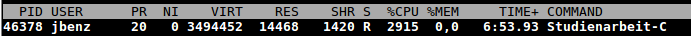
\includegraphics[width=0.7\textwidth]{../images/Benz/screenshot_top.png} %Screenshot top
	\caption{Eintrag mit Prozessorauslastung der x86-Implementierung} 
	\label{fig:conv_layer_seriell}
\end{figure}
 
\end{document}